% vim: set spell spelllang=en tw=100 et sw=4 sts=4 foldmethod=marker foldmarker={{{,}}} :

\documentclass[aspectratio=169,compress,10pt]{beamer}

\usepackage{tikz}
\usepackage{xcolor}
\usepackage{complexity}
\usepackage{hyperref}
\usepackage{microtype}
\usepackage{amsmath}                   % \operatorname
\usepackage{amsfonts}                  % \mathcal
\usepackage{amssymb}                   % \nexists
\usepackage[vlined]{algorithm2e} % algorithms
\usepackage{centernot}
\usepackage{listings}
\usepackage{csquotes}
\usepackage{fancyvrb}
\usepackage{bussproofs}
\usepackage{multicol}
\usepackage{booktabs}
\usepackage{mathtools}
\usepackage{pifont}
\usepackage{marvosym}
\usepackage{cancel}

\usefonttheme{professionalfonts}

\usetikzlibrary{shapes, arrows, shadows, calc, positioning, fit}
\usetikzlibrary{decorations.pathreplacing, decorations.pathmorphing, shapes.misc}
\usetikzlibrary{tikzmark, backgrounds}
\usetikzlibrary{trees, overlay-beamer-styles}
\usetikzlibrary{backgrounds, scopes, graphs, graphs.standard, shapes.geometric}
\usetikzlibrary{shapes.multipart, arrows, arrows.meta, decorations, decorations.markings}

\tikzset{processarrow/.style={->, very thick, decorate, decoration={snake, post length=0.5mm}}}
\tikzset{brace/.style={decorate, decoration={brace}, very thick}}

\definecolor{uofguniversityblue}{rgb}{0, 0.219608, 0.396078}
\definecolor{uofgheather}{rgb}{0.356863, 0.32549, 0.490196}
\definecolor{uofgaquamarine}{rgb}{0.603922, 0.72549, 0.678431}
\definecolor{uofgslate}{rgb}{0.309804, 0.34902, 0.380392}
\definecolor{uofgrose}{rgb}{0.823529, 0.470588, 0.709804}
\definecolor{uofgmocha}{rgb}{0.709804, 0.564706, 0.47451}
\definecolor{uofgsandstone}{rgb}{0.321569, 0.278431, 0.231373}
\definecolor{uofgforest}{rgb}{0, 0.2, 0.129412}
\definecolor{uofglawn}{rgb}{0.517647, 0.741176, 0}
\definecolor{uofgcobalt}{rgb}{0, 0.615686, 0.92549}
\definecolor{uofgturquoise}{rgb}{0, 0.709804, 0.819608}
\definecolor{uofgsunshine}{rgb}{1.0, 0.862745, 0.211765}
\definecolor{uofgpumpkin}{rgb}{1.0, 0.72549, 0.282353}
\definecolor{uofgthistle}{rgb}{0.584314, 0.070588, 0.447059}
\definecolor{uofgrust}{rgb}{0.603922, 0.227451, 0.023529}
\definecolor{uofgburgundy}{rgb}{0.490196, 0.133333, 0.223529}
\definecolor{uofgpillarbox}{rgb}{0.701961, 0.047059, 0}
\definecolor{uofglavendar}{rgb}{0.356863, 0.301961, 0.580392}
\definecolor{uofgleaf}{rgb}{0, 0.517647, 0.239216}

% {{{ theme things
\useoutertheme[footline=authortitle]{miniframes}
\useinnertheme{rectangles}

\setbeamerfont{block title}{size={}}
\setbeamerfont{title}{size=\large,series=\bfseries}
\setbeamerfont{section title}{size=\large,series=\mdseries}
\setbeamerfont{author}{size=\normalsize,series=\mdseries}
\setbeamercolor*{structure}{fg=uofguniversityblue}
\setbeamercolor*{palette primary}{use=structure,fg=black,bg=white}
\setbeamercolor*{palette secondary}{use=structure,fg=white,bg=uofgcobalt}
\setbeamercolor*{palette tertiary}{use=structure,fg=white,bg=uofguniversityblue}
\setbeamercolor*{palette quaternary}{fg=white,bg=black}
\setbeamercolor{block body}{bg=structure!10}
\setbeamercolor{block title}{bg=structure,fg=white}
\setbeamertemplate{blocks}[rounded]
\setbeamercolor*{titlelike}{parent=palette primary}

\beamertemplatenavigationsymbolsempty
\setbeamersize{text margin left=0.5cm}
\setbeamersize{text margin right=0.5cm}

\setbeamertemplate{title page}
{
    \begin{tikzpicture}[remember picture, overlay]
        \node at (current page.north west) {
            \begin{tikzpicture}[remember picture, overlay]
                \fill [fill=uofguniversityblue, anchor=north west] (0, 0) rectangle (\paperwidth, -2.6cm);
            \end{tikzpicture}
        };

        \node (logo) [anchor=north east, shift={(-0.8cm,-0.2cm)}] at (current page.north east) {
            
\includegraphics[keepaspectratio=true,scale=0.5]{../../images/UoG_keyline.pdf}
        };

        \node (logo2) [anchor=north, below=0.2cm of logo.south] {
            
\includegraphics[keepaspectratio=true,scale=0.1]{../../images/RAEngWhite.pdf}
        };

        \coordinate (logos) at ($(logo.south)!0.5!(logo2.north)$);

        \node [anchor=west, xshift=0.8cm] at (current page.west |- logos) {
            \begin{minipage}{0.65\paperwidth}\raggedright
                {\usebeamerfont{title}\usebeamercolor[white]{}\inserttitle}\\[0.2cm]
                {\usebeamerfont{author}\usebeamercolor[white]{}\insertauthor}
            \end{minipage}
        };
    \end{tikzpicture}
}

\setbeamertemplate{section page}
{
    \begin{centering}
        \begin{beamercolorbox}[sep=12pt,center]{part title}
            \usebeamerfont{section title}\insertsection\par
        \end{beamercolorbox}
    \end{centering}
}

\newcommand{\frameofframes}{/}
\newcommand{\setframeofframes}[1]{\renewcommand{\frameofframes}{#1}}

\makeatletter
\setbeamertemplate{footline}
{%
    \begin{beamercolorbox}[colsep=1.5pt]{upper separation line foot}
    \end{beamercolorbox}
    \begin{beamercolorbox}[ht=2.5ex,dp=1.125ex,%
        leftskip=.3cm,rightskip=.3cm plus1fil]{title in head/foot}%
        {\usebeamerfont{title in head/foot}\insertshorttitle}%
        \hspace{0.22\textwidth}%
        {\usebeamerfont{author in head/foot}\insertshortauthor}%
        \hfill%
        {\usebeamerfont{frame number}\usebeamercolor[fg]{frame number}\insertframenumber~\frameofframes~\inserttotalframenumber}
    \end{beamercolorbox}%
    \begin{beamercolorbox}[colsep=1.5pt]{lower separation line foot}
    \end{beamercolorbox}
}

\makeatletter
\setbeamertemplate{mini frame}
{%
  \begin{pgfpicture}{0pt}{0pt}{.04cm}{.04cm}
    \pgfpathcircle{\pgfpoint{0.04cm}{0.04cm}}{0.04cm}
    \pgfusepath{fill,stroke}
  \end{pgfpicture}%
}
\setbeamertemplate{mini frame in current subsection}
{%
  \begin{pgfpicture}{0pt}{0pt}{.04cm}{.04cm}
    \pgfpathcircle{\pgfpoint{0.04cm}{0.04cm}}{0.04cm}
    \pgfsetfillcolor{section in head/foot.bg}
    \pgfusepath{fill,stroke}
  \end{pgfpicture}%
}

\setbeamersize{mini frame size=0.10cm, mini frame offset=0.06cm}
\makeatother

\makeatletter
\newenvironment{nearlyplainframe}[2][]{
    \def\beamer@entrycode{\vspace*{-\headheight}\vspace*{3pt}}
    \setbeamertemplate{headline}
    {%
        \begin{beamercolorbox}[colsep=1.5pt]{upper separation line head}
        \end{beamercolorbox}
        \begin{beamercolorbox}[ht=0.5ex,dp=0.125ex,%
            leftskip=.3cm,rightskip=.3cm plus1fil]{title in head/foot}%
        \end{beamercolorbox}%
        \begin{beamercolorbox}[ht=0.5ex,dp=0.125ex,%
            leftskip=.3cm,rightskip=.3cm plus1fil]{author in head/foot}%
        \end{beamercolorbox}%
        \begin{beamercolorbox}[colsep=1.5pt]{lower separation line head}
        \end{beamercolorbox}
        \vspace*{\headheight}
    }

    \setbeamertemplate{footline}
    {%
        \begin{beamercolorbox}[colsep=1.5pt]{upper separation line foot}
        \end{beamercolorbox}
        \begin{beamercolorbox}[ht=0.5ex,dp=0.125ex,%
            leftskip=.3cm,rightskip=.3cm plus1fil]{author in head/foot}%
        \end{beamercolorbox}%
        \begin{beamercolorbox}[ht=0.5ex,dp=0.125ex,%
            leftskip=.3cm,rightskip=.3cm plus1fil]{title in head/foot}%
        \end{beamercolorbox}%
        \begin{beamercolorbox}[colsep=1.5pt]{lower separation line foot}
        \end{beamercolorbox}
    }

    \begin{frame}[#1]{#2}
    }{
    \end{frame}
}
\makeatother

% }}}

\tikzstyle{state} = [inner sep=1pt]
\tikzstyle{infeasible} = [color=uofgpillarbox]
\tikzstyle{dominated} = [color=uofgcobalt]
\tikzstyle{backwards} = []
\tikzstyle{accept} = [solid, thick]
\tikzstyle{reject} = [dotted, thick]
\tikzstyle{forced} = [color=uofglawn]
\tikzstyle{domination} = [dashed, thick, ->, color=uofgcobalt]

\newcommand{\set}[1]{\{ #1 \}}
\newcommand{\setsize}[1]{{\left|#1\right|}}

\newcommand{\solvernameformat}[1]{\textit{#1}}
\newcommand{\toolformat}[1]{\textit{#1}}
\newcommand{\proofsystemformat}[1]{\textsc{#1}\@}

\newcommand{\veripb}{\toolformat{VeriPB}\xspace}
\renewcommand{\veripb}{\proofsystemformat{VeriPB}\xspace}
\newcommand\veripbid[1]{\alertred{#1}}
\newcommand\veripbConstraint[1]{\alertblue{#1}}

\newcommand{\neighbourhood}{\operatorname{N}}
\newcommand{\vertexset}{\operatorname{V}}
\newcommand{\degree}{\operatorname{deg}}

\author{Ciaran McCreesh}
\title{Algorithms You Can Trust}

\begin{document}

{
    \usebackgroundtemplate{
        \tikz[overlay, remember picture]
        \node[at=(current page.south), anchor=south, inner sep=0pt, yshift=-1.4cm]{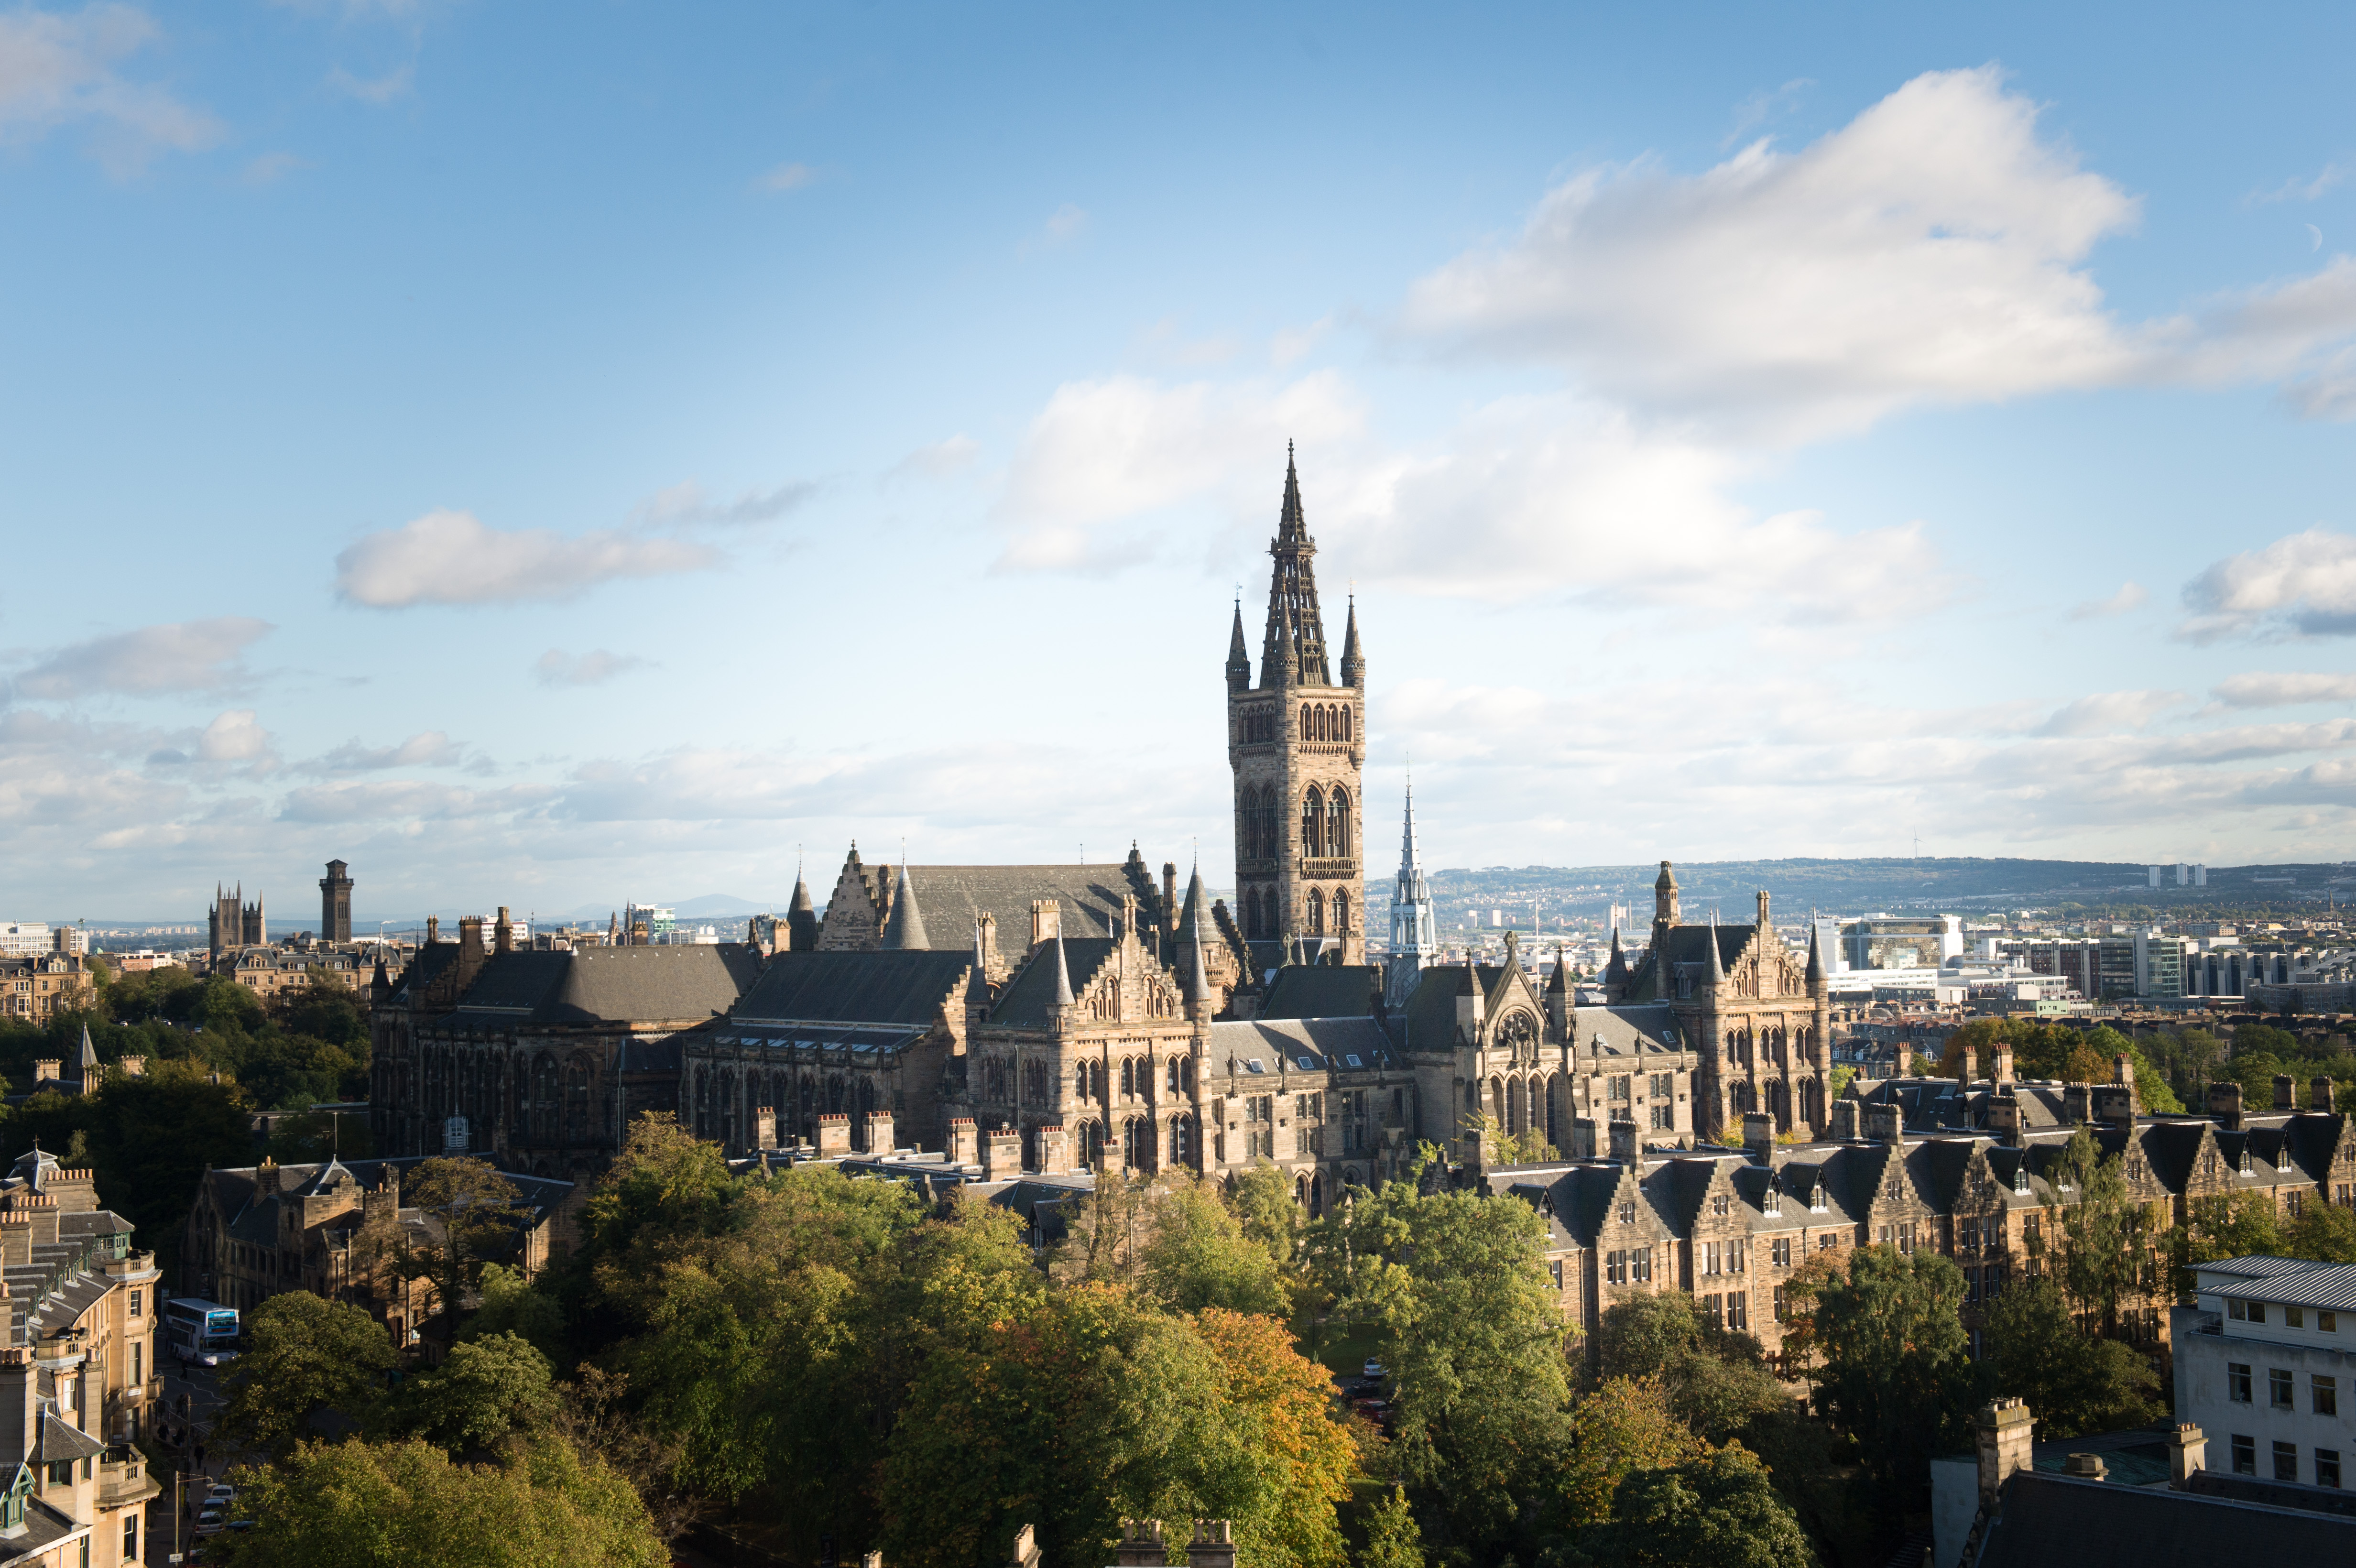
\includegraphics[keepaspectratio=true, width=\paperwidth]{../../images/background.jpg}};
    }
    \begin{frame}[plain,noframenumbering]
        \titlepage
    \end{frame}
}

\begin{frame}{Constraint Programming}
    \begin{itemize}
        \item A declarative way of specifying hard problems.
        \item \textbf{Variables} have \textbf{domains} of possible \textbf{values}.
            \begin{itemize}
                \item Typically, finite subsets of the integers.
            \end{itemize}
        \item \textbf{Constraints} specify restrictions on what values variables can take.
            \begin{itemize}
                \item Lots of different types.
            \end{itemize}
        \item Want to find a way of giving each variable a value from its domain, respecting all
            constraints.
            \begin{itemize}
                \item Or find the best way of doing so, maximising an objective variable.
            \end{itemize}
        \item A \textbf{solver} finds us the answer.
            \begin{itemize}
                \item A well-engineered suite of intelligent reasoning and search algorithms.
            \end{itemize}
    \end{itemize}
\end{frame}

\begin{frame}{The Most Famous Constraint Satisfaction Problem}
    \begin{center}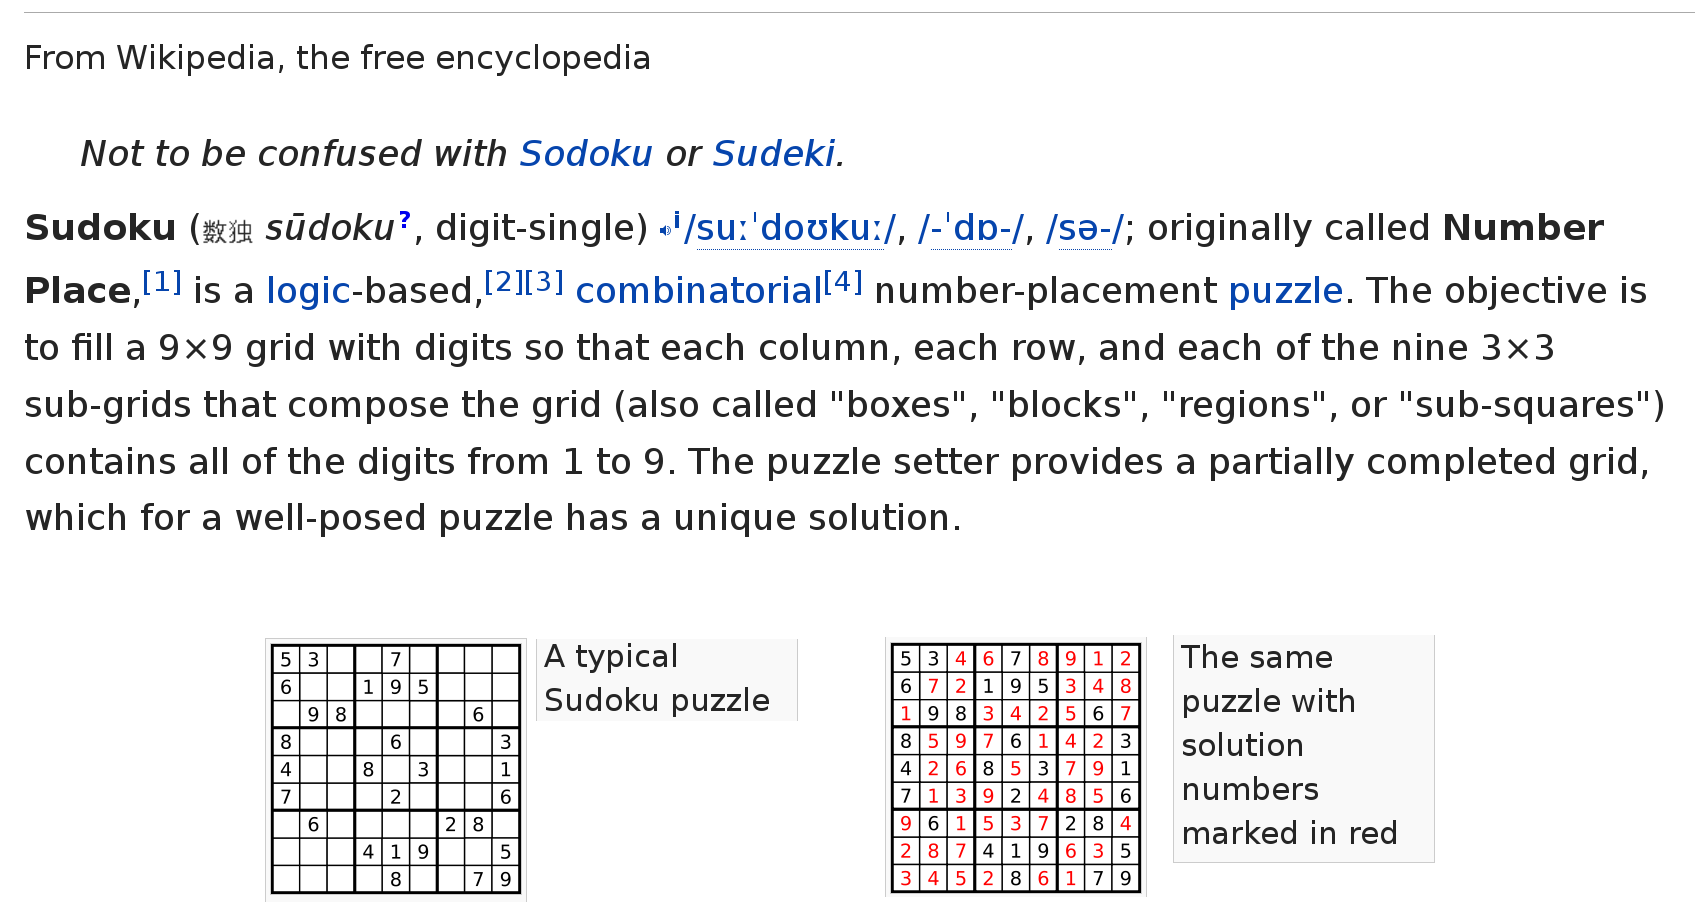
\includegraphics[scale=0.18]{sudoku.png}\end{center}
\end{frame}

\newcommand{\truck}[1]{\raisebox{-2pt}{
    \begin{tikzpicture}[scale=0.5, inner sep=0pt, outer sep=0pt]
        \path[fill=uofgsandstone] (0.9525, -0.7144).. controls (0.9525, -0.7728) and (0.9051, -0.8202) .. (0.8467, -0.8202) -- (0.1058, -0.8202).. controls (0.0474, -0.8202) and (0.0, -0.7728) .. (0.0, -0.7144) -- (0.0, -0.635).. controls (0.0, -0.5766) and (0.0474, -0.5292) .. (0.1058, -0.5292) -- (0.8467, -0.5292).. controls (0.9051, -0.5292) and (0.9525, -0.5766) .. (0.9525, -0.635) -- (0.9525, -0.7144) -- cycle;
        \path[fill=uofgsandstone!60!white] (0.5027, -0.344) -- (0.4768, -0.3175) -- (0.1891, -0.3175).. controls (0.1058, -0.3175) and (0.0794, -0.3704) .. (0.0794, -0.3704) -- (0.0, -0.5281) -- (0.0, -0.6615) -- (0.5027, -0.6615) -- (0.5027, -0.344) -- cycle;
        \path[fill=uofgsandstone!40!white] (0.2381, -0.5292) -- (0.0529, -0.5292) -- (0.1058, -0.4233) -- (0.2381, -0.3704) -- (0.2381, -0.5292) -- cycle;
        \path[fill=uofgsandstone!40!white] (0.2381, -0.8202) circle (0.1058cm);
        \path[fill=black] (0.2381, -0.8202) circle (0.0529cm);
        \path[fill=uofgsandstone!40!white] (0.7144, -0.8202) circle (0.1058cm);
        \path[fill=black] (0.7144, -0.8202) circle (0.0529cm);
        \path[fill=#1] (0.8467, -0.2117) -- (0.4498, -0.2117).. controls (0.3913, -0.2117) and (0.344, -0.2591) .. (0.344, -0.3175) -- (0.344, -0.6615) -- (0.9525, -0.6615) -- (0.9525, -0.3175).. controls (0.9525, -0.2591) and (0.9051, -0.2117) .. (0.8467, -0.2117) -- cycle;
    \end{tikzpicture}}
}

\newcommand{\parcel}{\raisebox{-2pt}{
\includegraphics[width=1.2em]{../../2024/a1-poster/parcel.pdf}\,}}
\newcommand{\trashpanda}{\raisebox{-2pt}{
\includegraphics[width=1.2em]{../../2024/a1-poster/trashpanda.pdf}\,}}
\newcommand{\bed}{\raisebox{-2pt}{
\includegraphics[width=1.2em]{../../2024/a1-poster/bed.pdf}\,}}
\newcommand{\chair}{\raisebox{-2pt}{
\includegraphics[width=1.2em]{../../2024/a1-poster/chair.pdf}\,}}
\newcommand{\tree}{\raisebox{-2pt}{
\includegraphics[width=1.2em]{../../2024/a1-poster/tree.pdf}\,}}
\newcommand{\present}{\raisebox{-2pt}{
\includegraphics[width=1.2em]{../../2024/a1-poster/present.pdf}\,}}
\newcommand{\laptop}{\raisebox{-2pt}{
\includegraphics[width=1.2em]{../../2024/a1-poster/laptop.pdf}\,}}
\newcommand{\drivera}{\raisebox{-2pt}{
\includegraphics[width=1.2em]{../../2024/a1-poster/driver1.pdf}\,}}
\newcommand{\driverb}{\raisebox{-2pt}{
\includegraphics[width=1.2em]{../../2024/a1-poster/driver2.pdf}\,}}

\begin{frame}{Industrial Applications}
    \begin{center}
    \begin{minipage}{8cm}
        \centering
        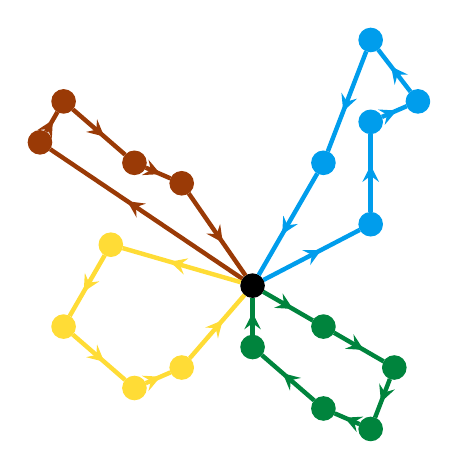
\begin{tikzpicture}
        \begin{scope}[yscale=2.6, xscale=3.0]
        \node (depot) [inner sep=3pt, draw, fill, circle] at (0,0) {};

        \node (RC1) [inner sep=3pt, draw, fill, circle, color=uofgcobalt] at (0.5,0.3) {};
        \node (RC2) [inner sep=3pt, draw, fill, circle, color=uofgcobalt] at (0.5,0.8) {};
        \node (RC3) [inner sep=3pt, draw, fill, circle, color=uofgcobalt] at (0.7,0.9) {};
        \node (RC4) [inner sep=3pt, draw, fill, circle, color=uofgcobalt] at (0.5,1.2) {};
        \node (RC5) [inner sep=3pt, draw, fill, circle, color=uofgcobalt] at (0.3,0.6) {};

        \begin{scope}[decoration={markings, mark=at position 0.6 with {\arrow{stealth}}}]
            \draw [postaction={decorate}, ultra thick, color=uofgcobalt] (depot) -- (RC1);
            \draw [postaction={decorate}, ultra thick, color=uofgcobalt] (RC1)   -- (RC2);
            \draw [postaction={decorate}, ultra thick, color=uofgcobalt] (RC2)   -- (RC3);
            \draw [postaction={decorate}, ultra thick, color=uofgcobalt] (RC3)   -- (RC4);
            \draw [postaction={decorate}, ultra thick, color=uofgcobalt] (RC4)   -- (RC5);
            \draw [postaction={decorate}, ultra thick, color=uofgcobalt] (RC5)   -- (depot);
        \end{scope}

        \node (RR1) [inner sep=3pt, draw, fill, circle, color=uofgrust] at (-0.9,0.7) {};
        \node (RR2) [inner sep=3pt, draw, fill, circle, color=uofgrust] at (-0.8,0.9) {};
        \node (RR3) [inner sep=3pt, draw, fill, circle, color=uofgrust] at (-0.5,0.6) {};
        \node (RR4) [inner sep=3pt, draw, fill, circle, color=uofgrust] at (-0.3,0.5) {};

        \begin{scope}[decoration={markings, mark=at position 0.6 with {\arrow{stealth}}}]
            \draw [postaction={decorate}, ultra thick, color=uofgrust] (depot) -- (RR1);
            \draw [postaction={decorate}, ultra thick, color=uofgrust] (RR1)   -- (RR2);
            \draw [postaction={decorate}, ultra thick, color=uofgrust] (RR2)   -- (RR3);
            \draw [postaction={decorate}, ultra thick, color=uofgrust] (RR3)   -- (RR4);
            \draw [postaction={decorate}, ultra thick, color=uofgrust] (RR4)   -- (depot);
        \end{scope}

        \node (RS1) [inner sep=3pt, draw, fill, circle, color=uofgsunshine] at (-0.6,0.2) {};
        \node (RS2) [inner sep=3pt, draw, fill, circle, color=uofgsunshine] at (-0.8,-0.2) {};
        \node (RS3) [inner sep=3pt, draw, fill, circle, color=uofgsunshine] at (-0.5,-0.5) {};
        \node (RS4) [inner sep=3pt, draw, fill, circle, color=uofgsunshine] at (-0.3,-0.4) {};

        \begin{scope}[decoration={markings, mark=at position 0.6 with {\arrow{stealth}}}]
            \draw [postaction={decorate}, ultra thick, color=uofgsunshine] (depot) -- (RS1);
            \draw [postaction={decorate}, ultra thick, color=uofgsunshine] (RS1)   -- (RS2);
            \draw [postaction={decorate}, ultra thick, color=uofgsunshine] (RS2)   -- (RS3);
            \draw [postaction={decorate}, ultra thick, color=uofgsunshine] (RS3)   -- (RS4);
            \draw [postaction={decorate}, ultra thick, color=uofgsunshine] (RS4)   -- (depot);
        \end{scope}

        \node (RL1) [inner sep=3pt, draw, fill, circle, color=uofgleaf] at (0.3,-0.2) {};
        \node (RL2) [inner sep=3pt, draw, fill, circle, color=uofgleaf] at (0.6,-0.4) {};
        \node (RL3) [inner sep=3pt, draw, fill, circle, color=uofgleaf] at (0.5,-0.7) {};
        \node (RL4) [inner sep=3pt, draw, fill, circle, color=uofgleaf] at (0.3,-0.6) {};
        \node (RL5) [inner sep=3pt, draw, fill, circle, color=uofgleaf] at (0,-0.3) {};

        \begin{scope}[decoration={markings, mark=at position 0.6 with {\arrow{stealth}}}]
            \draw [postaction={decorate}, ultra thick, color=uofgleaf] (depot) -- (RL1);
            \draw [postaction={decorate}, ultra thick, color=uofgleaf] (RL1)   -- (RL2);
            \draw [postaction={decorate}, ultra thick, color=uofgleaf] (RL2)   -- (RL3);
            \draw [postaction={decorate}, ultra thick, color=uofgleaf] (RL3)   -- (RL4);
            \draw [postaction={decorate}, ultra thick, color=uofgleaf] (RL4)   -- (RL5);
            \draw [postaction={decorate}, ultra thick, color=uofgleaf] (RL5)   -- (depot);
        \end{scope}
        \end{scope}
    \end{tikzpicture}
\end{minipage}\begin{minipage}{12cm}
    \truck{uofgrust} \drivera\driverb: \bed\parcel\chair\parcel

    \medskip

    \truck{uofgcobalt} \driverb\drivera:
    \chair\trashpanda\parcel\parcel\present


    \medskip

    \truck{uofgsunshine} \driverb\driverb: \tree\parcel\chair\present

    \medskip

    \truck{uofgleaf} \drivera\phantom{\drivera}:
    \parcel\parcel\laptop\parcel\parcel
\end{minipage}
\end{center}
\end{frame}

\begin{frame}{Subgraph Isomorphism}
    \only<1-8>{
    \centering
    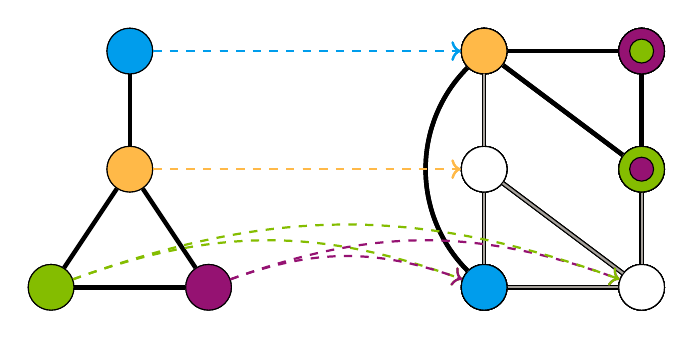
\begin{tikzpicture}
        \node <1> [draw, circle, fill=white, inner sep=4pt, font=\bfseries] (Na) at (1,  0) {\vphantom{1}};
        \node <1> [draw, circle, fill=white, inner sep=4pt, font=\bfseries] (Nb) at (1, -1.5) {\vphantom{1}};
        \node <1> [draw, circle, fill=white, inner sep=4pt, font=\bfseries] (Nc) at (0, -3) {\vphantom{1}};
        \node <1> [draw, circle, fill=white, inner sep=4pt, font=\bfseries] (Nd) at (2, -3) {\vphantom{1}};

        \node <2-8> [draw, circle, fill=uofgcobalt, inner sep=4pt, font=\bfseries] (Na) at (1,  0) {\vphantom{1}};
        \node <2-8> [draw, circle, fill=uofgpumpkin, inner sep=4pt, font=\bfseries] (Nb) at (1, -1.5) {\vphantom{1}};
        \node <2-8> [draw, circle, fill=uofglawn, inner sep=4pt, font=\bfseries] (Nc) at (0, -3) {\vphantom{1}};
        \node <2-8> [draw, circle, fill=uofgthistle, inner sep=4pt, font=\bfseries] (Nd) at (2, -3) {\vphantom{1}};

        \draw [ultra thick] (Na) -- (Nb);
        \draw [ultra thick] (Nb) -- (Nc);
        \draw [ultra thick] (Nc) -- (Nd);
        \draw [ultra thick] (Nb) -- (Nd);

        \node <1> [draw, circle, fill=white, inner sep=4pt, font=\bfseries] (N1) at (5.5,  0) {\vphantom{1}};
        \node <1> [draw, circle, fill=white, inner sep=4pt, font=\bfseries] (N2) at (7.5,  0) {\vphantom{1}};
        \node <1> [draw, circle, fill=white, inner sep=4pt, font=\bfseries] (N3) at (5.5, -1.5) {\vphantom{1}};
        \node <1> [draw, circle, fill=white, inner sep=4pt, font=\bfseries] (N4) at (7.5, -1.5) {\vphantom{1}};
        \node <1> [draw, circle, fill=white, inner sep=4pt, font=\bfseries] (N5) at (5.5, -3) {\vphantom{1}};
        \node <1> [draw, circle, fill=white, inner sep=4pt, font=\bfseries] (N6) at (7.5, -3) {\vphantom{1}};

        \node <2> [draw, circle, fill=uofgcobalt, inner sep=4pt, font=\bfseries] (N1) at (5.5,  0) {\vphantom{1}};
        \node <2> [draw, circle, fill=white, inner sep=4pt, font=\bfseries] (N2) at (7.5,  0) {\vphantom{1}};
        \node <2> [draw, circle, fill=uofgpumpkin, inner sep=4pt, font=\bfseries] (N3) at (5.5, -1.5) {\vphantom{1}};
        \node <2> [draw, circle, fill=white, inner sep=4pt, font=\bfseries] (N4) at (7.5, -1.5) {\vphantom{1}};
        \node <2> [draw, circle, fill=uofglawn, inner sep=4pt, font=\bfseries] (N5) at (5.5, -3) {\vphantom{1}};
        \node <2> [draw, circle, fill=uofgthistle, inner sep=4pt, font=\bfseries] (N6) at (7.5, -3) {\vphantom{1}};

        \node <3> [draw, circle, fill=uofgcobalt, inner sep=4pt, font=\bfseries] (N1) at (5.5,  0) {\vphantom{1}};
        \node <3> [draw, circle, fill=white, inner sep=4pt, font=\bfseries] (N2) at (7.5,  0) {\vphantom{1}};
        \node <3> [draw, circle, fill=uofgpumpkin, inner sep=4pt, font=\bfseries] (N3) at (5.5, -1.5) {\vphantom{1}};
        \node <3> [draw, circle, fill=white, inner sep=4pt, font=\bfseries] (N4) at (7.5, -1.5) {\vphantom{1}};
        \node <3> [draw, circle, fill=uofgthistle, inner sep=4pt, font=\bfseries] (N5) at (5.5, -3) {\vphantom{1}};
        \node <3> [draw, circle, fill=uofglawn, inner sep=4pt, font=\bfseries] (N6) at (7.5, -3) {\vphantom{1}};

        \node <4> [draw, circle, fill=uofglawn, inner sep=4pt, font=\bfseries] (N1) at (5.5,  0) {\vphantom{1}};
        \node <4> [draw, circle, fill=uofgthistle, inner sep=1pt, font=\bfseries] (N1b) at (5.5,  0) {\vphantom{1}};
        \node <4> [draw, circle, fill=uofgthistle, inner sep=4pt, font=\bfseries] (N2) at (7.5,  0) {\vphantom{1}};
        \node <4> [draw, circle, fill=uofglawn, inner sep=1pt, font=\bfseries] (N2b) at (7.5,  0) {\vphantom{1}};
        \node <4> [draw, circle, fill=white, inner sep=4pt, font=\bfseries] (N3) at (5.5, -1.5) {\vphantom{1}};
        \node <4> [draw, circle, fill=uofgpumpkin, inner sep=4pt, font=\bfseries] (N4) at (7.5, -1.5) {\vphantom{1}};
        \node <4> [draw, circle, fill=white, inner sep=4pt, font=\bfseries] (N5) at (5.5, -3) {\vphantom{1}};
        \node <4> [draw, circle, fill=uofgcobalt, inner sep=4pt, font=\bfseries] (N6) at (7.5, -3) {\vphantom{1}};

        \node <5> [draw, circle, fill=uofgpumpkin, inner sep=4pt, font=\bfseries] (N1) at (5.5,  0) {\vphantom{1}};
        \node <5> [draw, circle, fill=uofgthistle, inner sep=4pt, font=\bfseries] (N2) at (7.5,  0) {\vphantom{1}};
        \node <5> [draw, circle, fill=uofglawn, inner sep=1pt, font=\bfseries] (N2b) at (7.5,  0) {\vphantom{1}};
        \node <5> [draw, circle, fill=uofgcobalt, inner sep=4pt, font=\bfseries] (N3) at (5.5, -1.5) {\vphantom{1}};
        \node <5> [draw, circle, fill=uofglawn, inner sep=4pt, font=\bfseries] (N4) at (7.5, -1.5) {\vphantom{1}};
        \node <5> [draw, circle, fill=uofgthistle, inner sep=1pt, font=\bfseries] (N4b) at (7.5, -1.5) {\vphantom{1}};
        \node <5> [draw, circle, fill=white, inner sep=4pt, font=\bfseries] (N5) at (5.5, -3) {\vphantom{1}};
        \node <5> [draw, circle, fill=white, inner sep=4pt, font=\bfseries] (N6) at (7.5, -3) {\vphantom{1}};

        \node <6> [draw, circle, fill=white, inner sep=4pt, font=\bfseries] (N1) at (5.5,  0) {\vphantom{1}};
        \node <6> [draw, circle, fill=white, inner sep=4pt, font=\bfseries] (N2) at (7.5,  0) {\vphantom{1}};
        \node <6> [draw, circle, fill=uofgthistle, inner sep=4pt, font=\bfseries] (N3) at (5.5, -1.5) {\vphantom{1}};
        \node <6> [draw, circle, fill=uofglawn, inner sep=1pt, font=\bfseries] (N3b) at (5.5, -1.5) {\vphantom{1}};
        \node <6> [draw, circle, fill=uofgcobalt, inner sep=4pt, font=\bfseries] (N4) at (7.5, -1.5) {\vphantom{1}};
        \node <6> [draw, circle, fill=uofglawn, inner sep=4pt, font=\bfseries] (N5) at (5.5, -3) {\vphantom{1}};
        \node <6> [draw, circle, fill=uofgthistle, inner sep=1pt, font=\bfseries] (N5b) at (5.5, -3) {\vphantom{1}};
        \node <6> [draw, circle, fill=uofgpumpkin, inner sep=4pt, font=\bfseries] (N6) at (7.5, -3) {\vphantom{1}};

        \node <7> [draw, circle, fill=uofgcobalt, inner sep=4pt, font=\bfseries] (N1) at (5.5,  0) {\vphantom{1}};
        \node <7> [draw, circle, fill=white, inner sep=4pt, font=\bfseries] (N2) at (7.5,  0) {\vphantom{1}};
        \node <7> [draw, circle, fill=uofglawn, inner sep=4pt, font=\bfseries] (N3) at (5.5, -1.5) {\vphantom{1}};
        \node <7> [draw, circle, fill=uofgthistle, inner sep=1pt, font=\bfseries] (N3b) at (5.5, -1.5) {\vphantom{1}};
        \node <7> [draw, circle, fill=white, inner sep=4pt, font=\bfseries] (N4) at (7.5, -1.5) {\vphantom{1}};
        \node <7> [draw, circle, fill=uofgpumpkin, inner sep=4pt, font=\bfseries] (N5) at (5.5, -3) {\vphantom{1}};
        \node <7> [draw, circle, fill=uofgthistle, inner sep=4pt, font=\bfseries] (N6) at (7.5, -3) {\vphantom{1}};
        \node <7> [draw, circle, fill=uofglawn, inner sep=1pt, font=\bfseries] (N6b) at (7.5, -3) {\vphantom{1}};

        \node <8> [draw, circle, fill=uofgpumpkin, inner sep=4pt, font=\bfseries] (N1) at (5.5,  0) {\vphantom{1}};
        \node <8> [draw, circle, fill=uofgthistle, inner sep=4pt, font=\bfseries] (N2) at (7.5,  0) {\vphantom{1}};
        \node <8> [draw, circle, fill=uofglawn, inner sep=1pt, font=\bfseries] (N2b) at (7.5,  0) {\vphantom{1}};
        \node <8> [draw, circle, fill=white, inner sep=4pt, font=\bfseries] (N3) at (5.5, -1.5) {\vphantom{1}};
        \node <8> [draw, circle, fill=uofglawn, inner sep=4pt, font=\bfseries] (N4) at (7.5, -1.5) {\vphantom{1}};
        \node <8> [draw, circle, fill=uofgthistle, inner sep=1pt, font=\bfseries] (N4b) at (7.5, -1.5) {\vphantom{1}};
        \node <8> [draw, circle, fill=uofgcobalt, inner sep=4pt, font=\bfseries] (N5) at (5.5, -3) {\vphantom{1}};
        \node <8> [draw, circle, fill=white, inner sep=4pt, font=\bfseries] (N6) at (7.5, -3) {\vphantom{1}};

        \draw <1> [thick, color=uofgsandstone!50] (N1) -- (N2);
        \draw <1> [thick, color=uofgsandstone!50] (N1) -- (N3);
        \draw <1> [thick, color=uofgsandstone!50] (N1) -- (N4);
        \draw <1> [thick, color=uofgsandstone!50] (N2) -- (N4);
        \draw <1> [thick, color=uofgsandstone!50] (N3) -- (N5);
        \draw <1> [thick, color=uofgsandstone!50] (N3) -- (N6);
        \draw <1> [thick, color=uofgsandstone!50] (N4) -- (N6);
        \draw <1> [thick, color=uofgsandstone!50] (N5) -- (N6);
        \draw <1> [thick, color=uofgsandstone!50] (N1) to [in=135, out=225] (N5);

        \draw <2-3> [thick, color=uofgsandstone!50] (N1) -- (N2);
        \draw <2-3> [ultra thick] (N1) -- (N3);
        \draw <2-3> [thick, color=uofgsandstone!50] (N1) -- (N4);
        \draw <2-3> [thick, color=uofgsandstone!50] (N2) -- (N4);
        \draw <2-3> [ultra thick] (N3) -- (N5);
        \draw <2-3> [ultra thick] (N3) -- (N6);
        \draw <2-3> [thick, color=uofgsandstone!50] (N4) -- (N6);
        \draw <2-3> [ultra thick] (N5) -- (N6);
        \draw <2-3> [thick, color=uofgsandstone!50] (N1) to [in=135, out=225] (N5);

        \draw <4> [ultra thick] (N1) -- (N2);
        \draw <4> [thick, color=uofgsandstone!50] (N1) -- (N3);
        \draw <4> [ultra thick] (N1) -- (N4);
        \draw <4> [ultra thick] (N2) -- (N4);
        \draw <4> [thick, color=uofgsandstone!50] (N3) -- (N5);
        \draw <4> [thick, color=uofgsandstone!50] (N3) -- (N6);
        \draw <4> [ultra thick] (N4) -- (N6);
        \draw <4> [thick, color=uofgsandstone!50] (N5) -- (N6);
        \draw <4> [thick, color=uofgsandstone!50] (N1) to [in=135, out=225] (N5);

        \draw <5> [ultra thick] (N1) -- (N2);
        \draw <5> [ultra thick] (N1) -- (N3);
        \draw <5> [ultra thick] (N1) -- (N4);
        \draw <5> [ultra thick] (N2) -- (N4);
        \draw <5> [thick, color=uofgsandstone!50] (N3) -- (N5);
        \draw <5> [thick, color=uofgsandstone!50] (N3) -- (N6);
        \draw <5> [thick, color=uofgsandstone!50] (N4) -- (N6);
        \draw <5> [thick, color=uofgsandstone!50] (N5) -- (N6);
        \draw <5> [thick, color=uofgsandstone!50] (N1) to [in=135, out=225] (N5);

        \draw <6> [thick, color=uofgsandstone!50] (N1) -- (N2);
        \draw <6> [thick, color=uofgsandstone!50] (N1) -- (N3);
        \draw <6> [thick, color=uofgsandstone!50] (N1) -- (N4);
        \draw <6> [thick, color=uofgsandstone!50] (N2) -- (N4);
        \draw <6> [ultra thick] (N3) -- (N5);
        \draw <6> [ultra thick] (N3) -- (N6);
        \draw <6> [ultra thick] (N4) -- (N6);
        \draw <6> [ultra thick] (N5) -- (N6);
        \draw <6> [thick, color=uofgsandstone!50] (N1) to [in=135, out=225] (N5);

        \draw <7> [thick, color=uofgsandstone!50] (N1) -- (N2);
        \draw <7> [thick, color=uofgsandstone!50] (N1) -- (N3);
        \draw <7> [thick, color=uofgsandstone!50] (N1) -- (N4);
        \draw <7> [thick, color=uofgsandstone!50] (N2) -- (N4);
        \draw <7> [ultra thick] (N3) -- (N5);
        \draw <7> [ultra thick] (N3) -- (N6);
        \draw <7> [thick, color=uofgsandstone!50] (N4) -- (N6);
        \draw <7> [ultra thick] (N5) -- (N6);
        \draw <7> [ultra thick] (N1) to [in=135, out=225] (N5);

        \draw <8> [ultra thick] (N1) -- (N2);
        \draw <8> [thick, color=uofgsandstone!50] (N1) -- (N3);
        \draw <8> [ultra thick] (N1) -- (N4);
        \draw <8> [ultra thick] (N2) -- (N4);
        \draw <8> [thick, color=uofgsandstone!50] (N3) -- (N5);
        \draw <8> [thick, color=uofgsandstone!50] (N3) -- (N6);
        \draw <8> [thick, color=uofgsandstone!50] (N4) -- (N6);
        \draw <8> [thick, color=uofgsandstone!50] (N5) -- (N6);
        \draw <8> [ultra thick] (N1) to [in=135, out=225] (N5);

        \draw <2> [thick, dashed, color=uofgcobalt, arrows=->] (Na) to (N1);
        \draw <2> [thick, dashed, color=uofgpumpkin, arrows=->] (Nb) to (N3);
        \draw <2> [thick, dashed, color=uofglawn, arrows=->] (Nc) to [out=20, in=160] (N5);
        \draw <2> [thick, dashed, color=uofgthistle, arrows=->] (Nd) to [out=20, in=160] (N6);

        \draw <3> [thick, dashed, color=uofgcobalt, arrows=->] (Na) to (N1);
        \draw <3> [thick, dashed, color=uofgpumpkin, arrows=->] (Nb) to (N3);
        \draw <3> [thick, dashed, color=uofglawn, arrows=->] (Nc) to [out=20, in=160] (N6);
        \draw <3> [thick, dashed, color=uofgthistle, arrows=->] (Nd) to [out=20, in=160] (N5);
    \end{tikzpicture}}

    \begin{itemize}
        \item Find the \textcolor{uofgcobalt}{pattern} inside the \textcolor{uofgcobalt}{target}.
        \item Applications in compilers, biochemistry, model checking, pattern recognition, \ldots
        \item Often want to find \emph{all} matches.
    \end{itemize}
\end{frame}

\begin{frame}{The Slide That Keeps Getting Me Into Trouble}
    2021 MiniZinc challenge: for 1.28\% of instances, wrong solutions were claimed.
    \\
    \begin{itemize}
        \item False claims of unsatisfiability.
        \item False claims of optimality.
        \item Infeasible solutions produced.
        \item Not limited to a single solver, problem, or constraint.
        \item Not even consistent---same solver on same hardware and same instance can give
            different results on different runs.
    \end{itemize}
\end{frame}

\begin{frame}{The World's Shortest Maths Paper}
    \begin{center}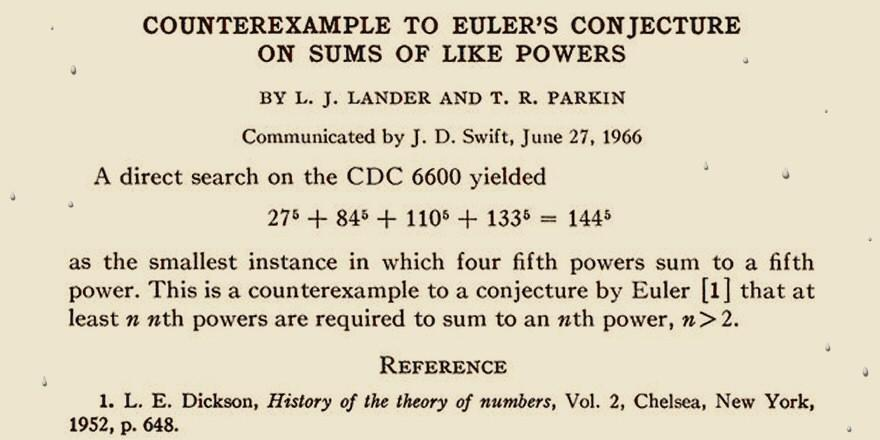
\includegraphics[scale=0.34]{shortest-math-paper.jpg}\end{center}
\end{frame}

\begin{frame}{Proof Logging}
    \vspace*{-1.0em}
    \begin{center}
        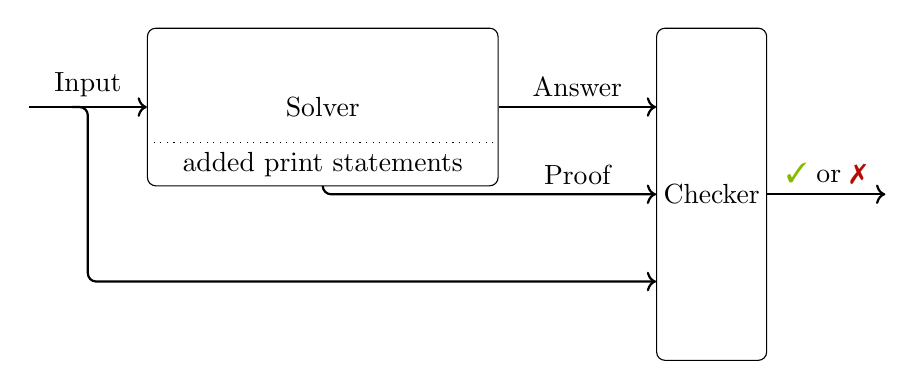
\begin{tikzpicture}
            \node (solver) [inner xsep=5em, inner ysep=2.5em, draw, rounded corners=3pt] { Solver };

            \node (checker) [right=2cm of solver.north east, anchor=north west, inner xsep=0.25em, draw, rounded corners=3pt, minimum height=12em, visible on=<3->] { Checker };

            \node (print) [anchor=south, above=0cm of solver.south, visible on=<2->] { added print statements };
            \draw [dotted, visible on=<2->] (solver.west|-print.north) -- (solver.east|-print.north);

            \draw [->, thick] (solver.east) -- (solver.east -| checker.west)
                coordinate [midway] (solutionmid) node [above, midway] { Answer };

            \draw [->, thick, rounded corners=3pt, visible on=<2->] (solver.south) -- (solver.south |- checker.west)
                -- (checker.west) coordinate [midway] (proofmid);

            \coordinate (prooflabel) at (proofmid-|solutionmid);
            \node [above=0cm of prooflabel, visible on=<2->] { Proof };

            \coordinate [right=1.5cm of checker.east] (verified);
            \draw [->, thick, visible on=<4->] (checker.east) -- (verified) node [above, midway] { \textcolor{uofglawn}{\ding{51}} or \textcolor{uofgpillarbox}{\ding{55}} };

            \coordinate [left=1.5cm of solver.west] (input);
            \draw [->, thick] (input) -- (solver.west) coordinate [midway] (inputmid) node [above, midway] { Input };

            \coordinate (checkerbotleft) at ($(checker.west)+($(checker.west)-(solver.east-|checker.west)$)$);

            \draw [->, thick, rounded corners=3pt, visible on=<3->] ($(inputmid)+(-0.2,0)$) -- (inputmid) -- (inputmid |- checkerbotleft) -- (checkerbotleft);
        \end{tikzpicture}
      \end{center}
    \vspace*{-0.7em}
  \begin{enumerate}
  \item<1->
    Run solver on problem input.
  \item<2->
    Solver also prints out a proof as part of its output.
  \item<3->
    Feed input + solution + proof to proof checker.
  \item<4->
    Verify that proof checker says solution is correct.
  \end{enumerate}
\end{frame}

\begin{frame}{Challenges}
    \begin{itemize}
        \item Proof system must be extremely simple, so we can trust the checker.
        \item But it must also capture rich reasoning that solvers use.
            \pause
        \item Surprisingly, cutting planes with dominance appears to satisfy both criteria.
    \end{itemize}

    \bigskip

    \begin{center}
        \url{https://gitlab.com/MIAOresearch/software/VeriPB}
    \end{center}
\end{frame}

{
    \usebackgroundtemplate{
        \tikz[overlay, remember picture]
        \node[at=(current page.south), anchor=south, yshift=-1cm, inner sep=0pt]{\includegraphics[keepaspectratio=true, width=\paperwidth]{../../images/background2.jpg}};
    }

    \begin{frame}[plain,noframenumbering]
        \begin{tikzpicture}[remember picture, overlay]
            \node at (current page.north west) {
                \begin{tikzpicture}[remember picture, overlay]
                    \fill [fill=uofguniversityblue, anchor=north west] (0, 0) rectangle (\paperwidth, -2.8cm);
                \end{tikzpicture}
            };

            \node (logo) [anchor=north east, shift={(-0.8cm,-0.2cm)}] at (current page.north east) {
                
\includegraphics[keepaspectratio=true,scale=0.5]{../../images/UoG_keyline.pdf}
            };

            \node (logo2) [anchor=north, below=0.2cm of logo.south] {
                
\includegraphics[keepaspectratio=true,scale=0.1]{../../images/RAEngWhite.pdf}
            };

            \coordinate (logos) at ($(logo.south)!0.5!(logo2.north)$);

            \node [anchor=west, xshift=0.8cm] at (current page.west |- logos) {
                \begin{minipage}{0.60\paperwidth}\raggedright
                    \textcolor{white}{\url{https://ciaranm.github.io/}} \\[0.3cm]
                    \textcolor{white}{\href{mailto:ciaran.mccreesh@glasgow.ac.uk}{\nolinkurl{ciaran.mccreesh@glasgow.ac.uk}}}
                \end{minipage}
            };
        \end{tikzpicture}
    \end{frame}
}

\end{document}

